\chapter{Testovanie}
\label{kap:testovanie}

V tejto kapitole zhrnieme výsledky z testovania aplikácie na cvičeniach kurzu Linux
pre používateľov.

\section{Priebeh testovania a funkčnosť systému}
\label{sec:funkcnost}

Systém sme nainštalovali na Linuxový server. Pred každým cvičením vyučujúci vytvoril
inštanciu cvičenia, nastavil interval jeho trvania, body za úspešné riešenia.
Spolu sa aplikácia testovala na desiatich cvičeniach. Študenti si stiahli z Moodle
GTA skript, ktorý si následne spustili na počítačoch v učebni.

Počas cvičenia nenastávali žiadne zdržania aplikácie, ktoré by spôsobili oneskorenú
vizualizáciu na strane klienta. Na poslednom cvičení sa vyskytla chyba pri spracovávaní
tela POST požiadavky, kedy GTA aplikácia zakódovala nesprávne riešenie a na strane
servera ho funkcia \verb'JSON.parse' nevedela spracovať. Preto sme sa nakoniec rozhodli
nahradiť \verb'urlencode' metódou \verb'base64'.


\section{Zhodnotenie aplikácie vyučujúcimi}
\label{sec:zhodnotenie}

Na konci semestra sme požiadali vyučujúcich o zhodnotenie aplikácie a jej prínos
na cvičeniach. Návrhy na možné vylepšenia uvádzame v sekcii~\ref{sec:futurework}.

Efektivita sa v porovnaní s minulým rokom zvýšila zásadne, nakoľko je možné preemptívne
zasiahuť a zastaviť sa pri študentovi, o ktorom je jasné, že je zaseknutý namiesto
toho, aby sme museli čakať, kedy sa prihlási. Tiež veľmi pomáha, že vieme odhadnúť,
kedy približne cvičenie skončí, kedže vidíme, v ktorom leveli sa nachádzajú jednotliví
študenti.

Druhým najvýraznejším prínosom aplikácie je možnosť klasifikovať riešenia.
Vyučujúcim to prinieslo lepší pohľad na rozmýšľanie študentov. Prednášajúcemu zas
možnosť sústrediť sa v prednáške na študentmi nepochopené učivo.

Vyučujúci taktiež hodnotia pozitívne implementáciu príkazu \verb'gta_help', vďaka
ktorej mohli študenti upozorniť vyučujúcich a požiadať o pomoc. My máme takto záznamy
v databáze a mohli by sme následne vyhodnotiť, pri ktorých úlohach študenti žiadali
najviac o pomoc. Avšak, tento príkaz mohli študenti používať až od polovice semestra.
Preto boli zvyknutý sa hlásiť klasicky zdvihnutím ruky a tento príkaz
využívali veľmi sporadicky. Z toho dôvodu nemáme relevantné dáta k vyhodnoteniu
potreby pomoci v jednotlivých úlohách.

\section{Výsledky}
\label{sec:vysledky}

Po skončenom cvičení máme prehľad o všetkých príkazoch, ktoré študenti odoslali.
Z nich vieme následne vyrobiť graf percentuálneho zastúpenia úspešných a neúspešných
príkazov (obrázky~\ref{img:histogram} a ~\ref{img:histogram2}).
Po prejdení myškou cez jednotlivé stĺpce vo webovom rozhraní sa zobrazí aj počet
úspešných a neúspešných príkazov. Na štvrtom cvičení použili študenti pri riešení
úlohy \textit{l01} 559 príkazov. Na deviatom cvičení to už bolo 1829. Je teda vidieť
značné zvýšenie náročnosti. Tabuľka~\ref{tab:exercises} zachytáva základný prehľad o
trvaní cvičení.\\

\begin{table}[h]
	\centering
	\begin{tabular}{|c||C{1.3cm}|C{1.8cm}|C{1.9cm}|C{1.6cm}|C{1.9cm}|C{1.7cm}|} 
		\hline
		& Počet úloh
		& Počet študentov
		& Priemerný počet príkazov
		& Medián počtu príkazov
		& Priemerný čas riešenia
		& Medián času riešenia \\
		\hline
		Cvičenie 1 & 7 & 54 & 11.52 & 11 & 00:19:52 & 00:21:09\\
		\hline
		Cvičenie 2 & 18 & 54 & 68.44 & 61 & 00:29:49 & 00:30:42\\
		\hline
		Cvičenie 3 & 10 & 54 & 76.70 & 71.50 & 01:02:17 & 01:06:55\\
		\hline
		Cvičenie 4 & 7 & 54 & 69.41 & 65 & 00:53:36 & 00:54:50\\
		\hline
		Cvičenie 5 & 6 & 52 & 36.53 & 33 & 00:53:40 & 00:53:08\\
		\hline
		Cvičenie 6 & 7 & 54 & 43.41 & 43 & 00:31:08 & 00:31:09\\
		\hline
		Cvičenie 7 & 5 & 53 & 52.15 & 48 & 00:38:43 & 00:39:15\\
		\hline
		Cvičenie 8 & 6 & 50 & 96.60 & 85 & 00:54:07 & 00:55:26\\
		\hline
		Cvičenie 9 & 5 & 51 & 99.39 & 97 & 01:12:21 & 01:09:47\\
		\hline
		Cvičenie 10 & 4 & 47 & 54.63 & 50 & 01:21:59 & 01:26:11\\
		\hline
	\end{tabular}
	\caption[Vyhodnotenie trvania cvičení]{Vyhodnotenie trvania cvičení}
	\label{tab:exercises}
\end{table}

Klasifikácia riešení metódou \textit{K-means} nám priniesla veľmi zaujímavé výsledky.
Pri testovaní zhlukovania príkazov sa špeciálne bigramy javia ako
lepšia reprezentácia vstupu. Pri príkazoch s nízkym počtom podpríkazov a argumentov
stačia aj unigramy. Niekedy je nutné spustiť algoritmus viackrát kvôli náhodnosti
výberu počiatočných centroidov.

Nižšie uvádzame príklady troch správnych riešení úlohy, v ktorej mali študenti v súbore 
nájsť definíciu funkcie, v ktorej sa nachádza slovo \textit{page}. Každé z riešení sa
dostalo do jedného z clusterov. V tabuľke~\ref{tab:distances} môžme vidieť vzdialenosti
medzi jednotlivými riešeniami.
\begin{enumerate}[label=(\alph*)]
	\item \verb'grep -n -i "def.*page[a-z^(]" test_cases.py > funkcia.txt'
	\item \verb'grep -n "def" test_cases.py | grep "page.*(" > funkcia.txt'
	\item \verb'cat test_cases.py | grep -n "def.*" | grep "page(" > funkcia.txt'
\end{enumerate}

\begin{table}[h]
	\centering
	\begin{tabular}{|c||c|c|} 
		\hline
		& Jaccardova vzdialenosť
		& Kosínusová vzdialenosť\\
		\hline
		Unigramy (a), (b) & 0.5 & 0.33184689521893906\\
		\hline
		Unigramy (a), (c) & 0.5454545454545454 & 0.37005921165128797\\
		\hline
		Unigramy (b), (c) & 0.4545454545454546 & 0.29289321881345254\\
		\Xhline{1.5pt}
		Špec. bigramy (a), (b) & 0.5 & 0.33184689521893906\\
		\hline
		Špec. bigramy (a), (c) & 0.6666666666666667 & 0.49604736932103044\\
		\hline
		Špec. bigramy (b), (c) & 0.5833333333333333 & 0.41074434901121050\\
		\hline
	\end{tabular}
	\caption[Porovnanie vzdialeností reprezentácií vstupov (a), (b), (c)]{Porovnanie vzdialeností reprezentácií vstupov (a), (b), (c)}
	\label{tab:distances}
\end{table}

Poďme sa ďalej pozrieť na úlohu, kde bolo treba vypísať posledný stĺpec zo súboru
\verb'/etc/passwd'. Prvé dve riešenia sa dostali do rovnakého clustera.

\begin{enumerate}[label={(\arabic*)}]
	\item \verb'grep "[^:]*$" -o /etc/passwd > zoznam.txt'
	\item \verb'grep "[^:]*$" -o /etc/passwd > ../zoznam.txt'
	\item \verb'cat /etc/passwd | grep -o "[^:]*$" > zoznam.txt'
\end{enumerate}

\begin{table}[h]
	\centering
	\begin{tabular}{|c||c|c|} 
		\hline
		& Jaccardova vzdialenosť
		& Kosínusová vzdialenosť\\
		\hline
		Unigramy (1), (2) & 0.2857142857142857 & 0.16666666666666652\\
		\hline
		Unigramy (1), (3) & 0.25 & 0.1339745962155613\\
		\hline
		Unigramy (2), (3) & 0.4444444444444444 & 0.2783121635129677\\
		\Xhline{1.5pt}
		Špec. bigramy (1), (2) & 0.2857142857142857 & 0.16666666666666652\\
		\hline
		Špec. bigramy (1), (3) & 0.5 & 0.3195861825602282\\
		\hline
		Špec. bigramy (2), (3) & 0.6363636363636364 & 0.45566894604818264\\
		\hline
	\end{tabular}
	\caption[Porovnanie vzdialeností reprezentácií vstupov (1), (2), (3)]{Porovnanie vzdialeností reprezentácií vstupov (1), (2), (3)}
	\label{tab:distances2}
\end{table}

V tomto prípade si môžeme v tabuľke~\ref{tab:distances2}
všimnúť, že vzdialenosti unigramových reprezentácií
(1) a (2) sú väčšie ako pri (1) a (3). My by sme však chceli, aby to bolo presne opačne
a príkazy (1) a (2) boli k sebe bližšie ako (1) a (3). Nami navrhnuté špeciálne bigramy
vyriešili tento problém, čo sa prejavilo aj na vzdialenostiach.
Vo všeobecnosti však nemusí platiť, že naše špeciálne bigramy sú vždy lepšie ako unigramy.
Preto sme sa v aplikácii rozhodli ponechať obidve možnosti a používateľ sa môže
rozhodnúť, ktorú použije. Taktiež, z výsledkov nie je úplne jasné, ktorá metrika
je lepšia. Vidíme iba, že Jaccardova vzdialenosť udáva väčšinou o pár stotín
väčšiu vzdialenosť.

Na obrázku~\ref{img:tsne} je ukážka zobrazenia riešení v 2D priestore pomocou
t-SNE, ktoré boli rozdelené do troch clusterov.

\begin{figure}[h]
	\centerline{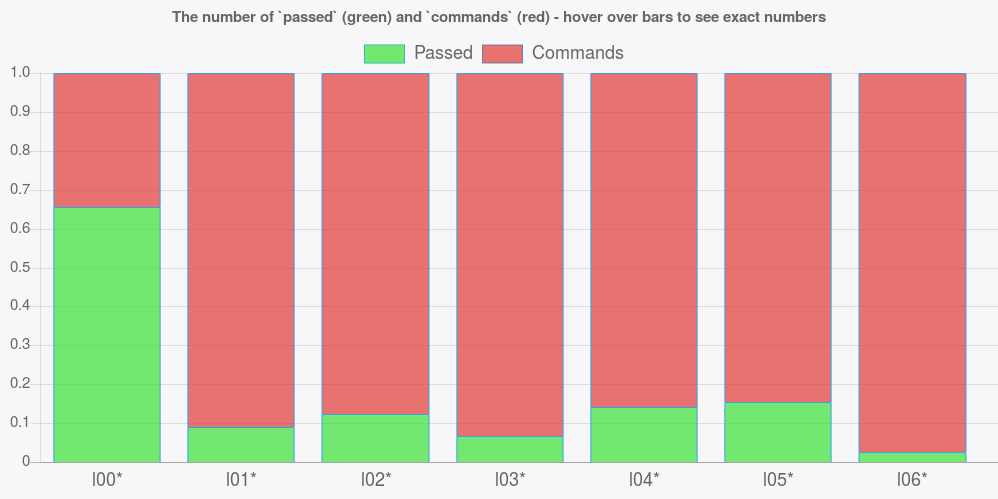
\includegraphics[width=1\textwidth]{images/histogram.png}}
	\caption[Percentuálne zastúpenie úspešných a neúspešných pokusov o riešenie]{Percentuálne zastúpenie úspešných a neúspešných pokusov o riešenie v rámci každej z úloh (cvičenie č. 4)}
	\label{img:histogram}
	
	\vspace{\baselineskip}
	\vspace{\baselineskip}
	
	\centerline{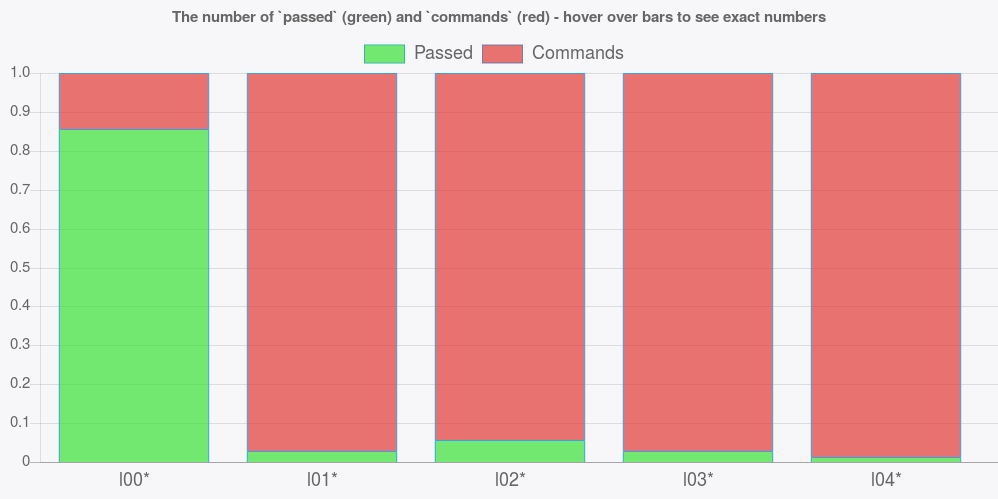
\includegraphics[width=1\textwidth]{images/histogram2.png}}
	\caption[Percentuálne zastúpenie úspešných a neúspešných pokusov o riešenie 2]{Percentuálne zastúpenie úspešných a neúspešných pokusov o riešenie v rámci každej z úloh (cvičenie č. 9)}
	\label{img:histogram2}
\end{figure}

\begin{sidewaysfigure}[h]
	\centerline{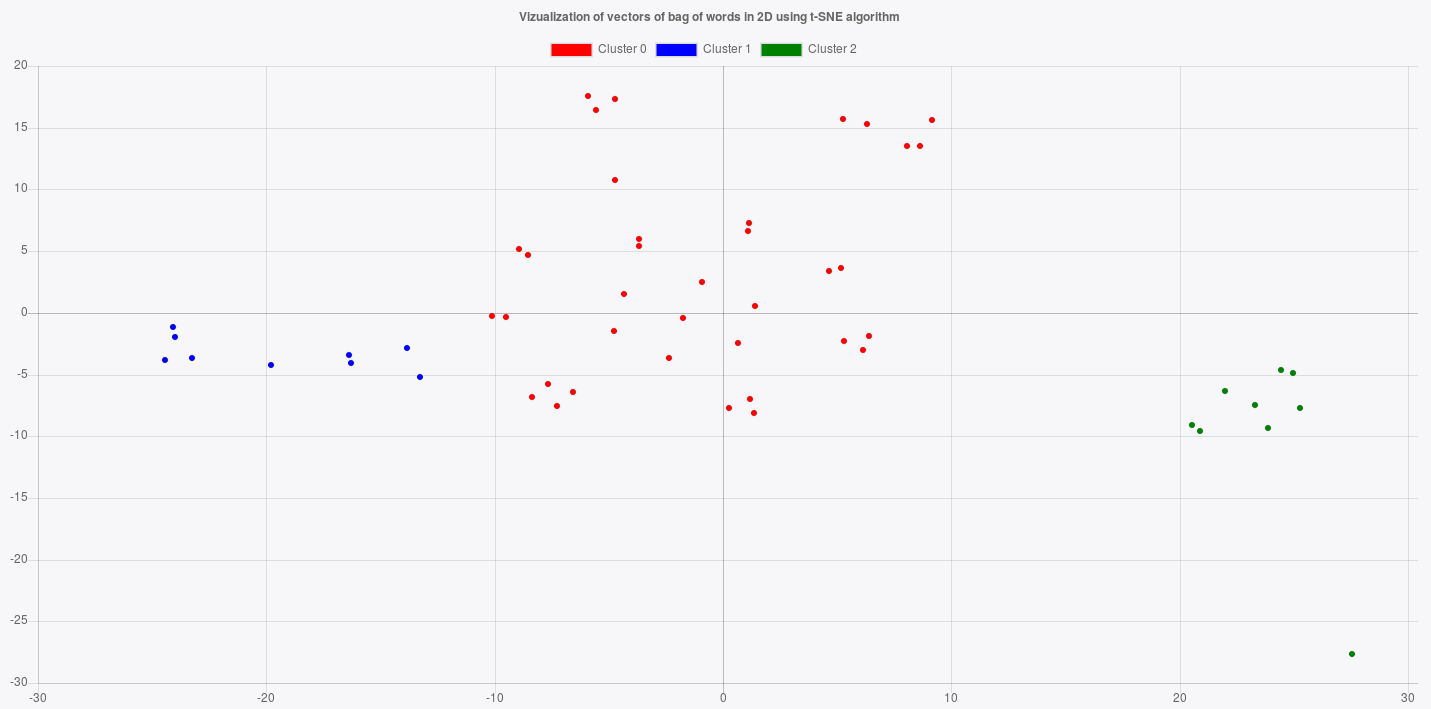
\includegraphics[width=1\textwidth]{images/tsnevizualizacia.png}}
	\caption[Vizualizácia vzdialeností riešení pomocou t-SNE]{Vizualizácia vzdialeností riešení pomocou t-SNE (3 clustery)}
	\label{img:tsne}
\end{sidewaysfigure}


